\chapter{Completed Work: Latent Factor Interpretation}

In this study, we introduce a method for generating explanations for the
output of matrix factorization systems by means of interpreting latent factors
with shadow models.

\section{Motivation}

Recommender systems that perform collaborative filtering via matrix
factorization are state-of-the-art in important application domains,
including movie and social
recommendations~\cite{koren2009matrix,facebook-cf}.
However, these models are difficult to interpret because they express
user preferences and item characteristics along a set of uninterpreted
latent factors trained from a sparse set of user ratings.

In order to interpret models that use uninterpreted latent factors, we
address three challenges.

The first challenge is that the latent factors are constants
uninterpretable to humans; any explanations in terms of these factors
would be unintelligible.
In order to address this problem, we learn a mapping from
interpretable features to these latent factors.
We then compose the mapping with the rest of the model. 
In our setting, we compose the interpretation of item latent factors
with user latent factors to make recommendations. 
We call the composed model, a \emph{shadow model}.

Our second challenge is that this composed shadow model still remains
too complex for direct interpretation.
However, since the shadow model expresses ratings in terms of
interpretable features, we can leverage existing model explanation
techniques~\cite{datta2016algorithmic,ribeiro2016lime}.
In particular, in this paper, we determine influential features using
an existing technique \cite{datta2016algorithmic}.
Note that the purpose of the shadow model is not to supplant the
recommender system, but to interpret its predictions.

The third challenge is maintaining correspondence between
interpretations and the models they explain.
Re-expression of a system via a shadow model does not guarantee that
the interpretations constructed from the shadow represent the
functioning of the original. 
In our approach, we substitute predicted item latent factors but keep
the remaining structure of the recommender system intact. 
Therefore the effects of the item factors on recommendations in the
shadow model are identical to those of the original. 
Demonstrating a level of accuracy in predicting both the latent
factors, and the resulting recommendations, we can claim that our
interpretations are meaningful because \textbf{the shadow model makes
  similar recommendations for similar reasons.}

\section{Method}

Our approach to interpreting recommender systems based on matrix factorization
comprises of two steps. First, we use publicly available interpretable features 
(i.e., metadata) about items as interpretable features
to predict latent factors of these items. We then compose these models
for predicting latent factors into models that predict the outcomes
for particular users. Second, this shadow model composed of predictors for the latent
factors is used to generate human-understandable explanations of outcomes
by identifying the most influential interpretable features.

The recommender system itself is trained on a MovieLens 20M data set
\cite{data-movielens}, that consists of $<user,movie,rating>$ tuples, where
rating is given as an integer value from 1 to 5, user is given by an anonymous
ID, and movie is given by an ID that is uniquely associated with the movie
title.

The metadata for the movies is assembled from multiple sources. MovieLens data
set itself contains data about movie genres and user-generated unstructured
tags. Then we incorporated the IMDB data set\cite{data-imdb}, that contains
information about user-generated movie keywords, directors, producers,
composers, and other data. Finally, we incorporated DBTropes\cite{data-dbtropes}
-- a machine-readable version of TV Tropes -- a wiki-based website that contains
descriptions of movies and other media in terms of commonly appearing patterns,
which they call ``tropes''. We have also tried incorporating more unstructured
user-generated data and using topic modeling to transform it into
machine-readable features, but this method has not increased the quality of
prediction and explanation substantially enough to be used.

We assume that we are given a matrix of interpretable attributes $A$, with
one row $\vect{a}_i$ for each item $i$. For each item latent factor $j$, we train
a predictor $f_j$  such that $f_j(\vect{a}_i) \approx \vect{i}_{ij}$.
Composing these predictors, the final predicted recommendation for a user $u$ and item $i$
can be approximated as follows:

\[\hat{r}_{ui} = \vect{u}_u\cdot\vect{i}_i = \sum_{j = 1}^k \vect{u}_{uj}\vect{i}_{ij} \approx
  \sum_{j = 1}^k \vect{u}_{uj}f_j(\vect{a}_i).
\]

Consequently, we use the composed model $\tilde{r}_u(\vect{a}) = \sum_{j = 1}^k
\vect{u}_{uj}f_j(\vect{a})$ as a model that predicts the outcomes of the system
for a movie with interpretable attributes $\vect{a}$ and user $u$. This shadow model
is more interpretable insofar as it maps interpretable attributes to
ratings. However, it is still fairly complex. Therefore, to interpret the
behavior of the shadow model $\tilde{r}_u$ on a point $\vect{a}$, we examine
the influences of interpretable attributes using QII.

We interpret the shadow model by measuring the quantitative input
influence of all metadata features

on its output.
This can be measured either on the output of a particular user-item
pair, in which case the question being answered is ``why were you
given this recommendation?''
or the entirety of the model's predictions for this user over all
items, in which case the measure would be answering ``what has the
model inferred about your preferences in general?''.
In its raw form, an interpretation takes the form of a list of
feature-influence pairs but can be naturally visualized as in
Figure~\ref{fig:results:qii}.

\begin{figure*}[t!]
  \centering
  \begin{subfigure}[t]{0.45\textwidth}
    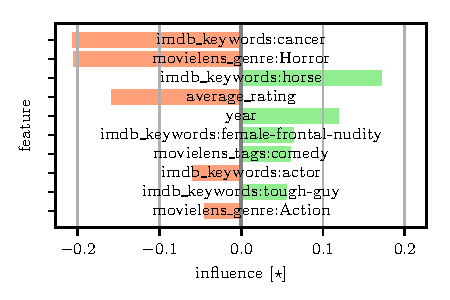
\includegraphics[width=3in]{figures/qii_user_7_movie_2713_real_data.pdf}
    \caption{User 7's recommendation about Lake Placid (1999)}
  \end{subfigure}~
  \begin{subfigure}[t]{0.45\textwidth}
    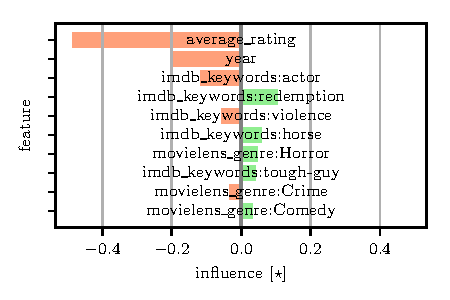
\includegraphics[width=3in]{figures/qii_user_21_movie_2713_real_data.pdf}
    \caption{User 21's recommendation about Lake Placid (1999)}
  \end{subfigure}

  \begin{subfigure}[t]{0.45\textwidth}
    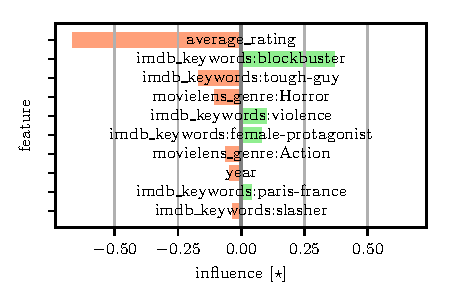
\includegraphics[width=3in]{figures/qii_user_7_movie_2720_real_data.pdf}
    \caption{User 7's recommendation about Inspector Gadget (1999)}
  \end{subfigure} ~
  \begin{subfigure}[t]{0.45\textwidth}
    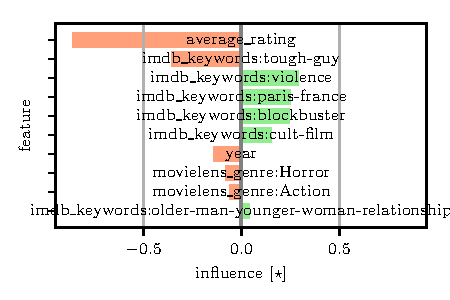
\includegraphics[width=3in]{figures/qii_user_21_movie_2720_real_data.pdf}
    \caption{User 21's recommendation about Inspector Gadget (1999)}
  \end{subfigure}


  \caption{\label{fig:results:qii}A sampling of QII-based
    recommendation interpretations based on shadow models over the
    MovieLens 20M dataset for User 7 (left) and User 21 (right).
  }
\end{figure*}


We measure the quality of the shadow model by computing the mean
absolute error of its predictions compared to the original model,
that we call \emph{baseline}.

Another metric of the quality of the shadow model is how close it
agrees with the original model on the latent factors themselves.
For each factor, we compute the mean absolute error (MAE) of latent
factor prediction. 
Averaging over all factors, we get a measure of the overall latent
factor agreement.


















The process of building a recommender system and interpreting its output goes
as follows:

\begin{enumerate}
	\item
		A matrix factorization model is trained on the MovieLens data
		set;
	\item
		After a matrix of movie latent factors is obtained, we treat
		each latent factor as the target variable to be predicted with
		a decision tree model from metadata features;
	\item
		Once we have built this model, we treat recommendations given by
		it as proxies for the real recommendations, and in order to see
		which metadata features are influential in a particular
		recommendation, we use the QII method and randomly perturb the
		values of metadata features and compare this counterfactual
		output to the original output;
	\item
		The features which affect the output the most are deemed the
		most influential.
\end{enumerate}

The shadow model can be evaluated in at least two ways: the quality of
prediction of individual latent factors (``latent factor agreement'') and the
quality of prediction of the end recommendation compared to the original model
(``observational agreement''). One might assume that these two metrics should
always correspond to each other; however, we have shown that it is not
necessarily the case, and one model can perform the best on latent factor
agreement, whereas another one can perform the best on observational agreement.

The explanation for a recommendation is given in the form of a vector that shows
for every metadata feature with non-zero influence its numeric influence
value, which also indicated whether the influence is positive of negative. This
vector can also be sorted by the absolute value of the influence into a ranked
list of the most influential features.

In order to numerically evaluate how accurate the explanations are, we generate
a data set of ratings that are assigned to movies by simulated users, each of
whom has a set of liked and disliked features, and the rating is determined by
their presence or absence for a given movie. Since the true list of features
that influence preferences of a particular user is known, every explanation can
be evaluated by how close to the top of the list of inferred influential
features the real ones are. We have shown that with a high statistical
significance, our method is consistently determining the influential features
better than random.

One piece of proposed work is to apply this method to course recommendations by
Coursera, with whom we are discussing the possibility of collaboration. The
usage of a recommendation system with good transparency properties could improve
both how much the users trust the system and how good the recommendations
given to them are.
